\documentclass[a4paper,10pt,twocolumn]{ltjsarticle}
\usepackage[haranoaji]{luatexja-preset}
\usepackage[top=18mm,bottom=20mm,left=17mm,right=17mm,columnsep=8mm]{geometry}
\usepackage{graphicx,booktabs,array,caption,enumitem,xcolor,tikz}
\usetikzlibrary{shapes.geometric}
\setlength{\parindent}{1\zw}
\renewcommand{\baselinestretch}{1.0}
\setlength{\parskip}{0pt}
\renewcommand{\thesection}{\arabic{section}.}
\renewcommand{\thesubsection}{\arabic{section}.\arabic{subsection}.}
\makeatletter
\renewcommand{\section}{\@startsection{section}{1}{\z@}{1.1\Cvs \@plus.4\Cdp \@minus.2\Cdp}{.5\Cvs \@plus.2\Cdp}{\normalfont\gtfamily\bfseries\large}}
\renewcommand{\subsection}{\@startsection{subsection}{2}{\z@}{.8\Cvs \@plus.3\Cdp \@minus.2\Cdp}{.3\Cvs \@plus.1\Cdp}{\normalfont\gtfamily\bfseries\normalsize}}
\makeatother
\captionsetup{font={small,sf},labelsep=space,justification=raggedright,singlelinecheck=false,skip=3pt}
\captionsetup[table]{position=top}
\setlist[itemize]{leftmargin=1.2\zw,itemsep=0pt,topsep=2pt,parsep=0pt}
\setlength{\textfloatsep}{8pt plus 2pt minus 2pt}
\setlength{\floatsep}{8pt plus 2pt minus 2pt}
\setlength{\intextsep}{8pt plus 2pt minus 2pt}
\pagestyle{plain}
\raggedbottom
\begin{document}
\twocolumn[{
\noindent\fbox{\gtfamily\small\ 生成AI論文\ }\par\medskip
\begin{center}
{\gtfamily\bfseries\LARGE 数学の男女の得点差は，国によってどう違うのか：PISA 2025の90の国・地域を並べる$^{\dagger}$}\par\medskip
{\gtfamily\bfseries\large 数学的リテラシーの男女得点差（男子−女子）の分布と日本の位置}\par\medskip
{\normalsize EduData調査研究グループ$^{*1}$・教育データサイエンス解析班$^{*2}$}\par
{\small オープン教育統計推進プロジェクト$^{*1}$・初等中等STEM教育データ基盤ユニット$^{*2}$}
\end{center}\smallskip
\noindent\begin{minipage}{\textwidth}\small PISA 2025の公表値を用い，数学的リテラシーの男女得点差（男子−女子）を90の国・地域で整理した．差は-27.2点から24.0点（単純平均8.04点，中央値9.05点）に分布し，男子のほうが高い国・地域は71，女子のほうが高いところは19であった．標準誤差の1.96倍を超える（おおよそ5\%水準）のは62（男子55，女子7）で，.05÷90の基準では44であった．日本は平均得点525.4点で5番目，差16.3点は大きい側から19番目だが，差の標準誤差5.7点は2番目に大きく，95\%信頼区間5.1〜27.5点は平均差を含むため，順位は確かではない．結果は国・地域の集計値の記述であり，個々の生徒の因果や理由は示さない．\par\smallskip
\noindent{\gtfamily キーワード：}PISA 2025，数学的リテラシー，男女得点差，国際比較\end{minipage}\medskip
}]
\let\thefootnote\relax
\footnotetext{\footnotesize 2026年10月執筆\\ $^{\dagger}$How Do Gender Gaps in Mathematics Differ by Country? Ranking 90 Countries and Economies in PISA 2025†\\ $^{*1}$ Open Education Data Project, Tokyo, Japan\quad $^{*2}$ Educational Data Science Unit, Tokyo, Japan}
\section{はじめに}
\subsection{研究の背景}
数学の成績の男女差は，国際的に長く論じられてきた．Hyde et al. (2008)は，数学の成績では男女の類似性が特徴的であると論じた．Lindberg et al. (2010)は男女差の新たな傾向をメタ分析で，Else-Quest et al. (2010)は男女差の国による違いをメタ分析で扱った．国による違いの背景として，Guiso et al. (2008)は文化と数学の男女差を，Spencer et al. (1999)はステレオタイプ脅威と女性の数学成績を論じたが，いずれも本研究のデータで検証できるものではない．Blickenstaff (2005)は，女性の理系キャリアをめぐる「漏れのある水路」か「ジェンダーフィルター」かを論じており，学校段階の得点差を進路の議論と結びつけて読むときの枠組みの一つになる．

PISAはOECDが実施する15歳の学習到達度調査で，PISA 2022の結果はOECD (2023)にまとめられている．本研究は，OECD (2026)が公表したPISA 2025の統計表のうち，副次的な分野である数学的リテラシーの男女得点差を，国・地域ごとに並べて記述する．
\subsection{リサーチクエスチョン}
本研究の目的は，PISA 2025の公表値から，数学的リテラシーの男女得点差（男子−女子）の国・地域による分布と日本の位置を記述することである．
\begin{itemize}
\item RQ1：数学の男女得点差（男子−女子）は，国・地域によってどのように分布し，日本はどこに位置するか．
\item RQ2：男女得点差が，標準誤差を考慮しても男子（または女子）のほうが高いと言える国・地域は，どれくらいあるか．
\end{itemize}
\section{調査対象および分析方法}
OECD (2026)の統計表から，数学的リテラシーの男女計・男子・女子の平均得点と，男女得点差（男子−女子）とその標準誤差を，90の国・地域について取り込んだ（OECD平均は除き，ウズベキスタンは欠測のため除いた）．アルバニア・カナダ・オランダ・ニュージーランド・ノルウェー・アメリカの6か国は，標本抽出基準についての注意（*）がある．分析単位は国・地域で，各国・地域を同じ重みで扱ったため，平均や中央値は人口で重みづけした値でもOECD平均でもない．差の正は男子のほうが高いことを示す．差の有無は，差の絶対値が標準誤差の1.96倍を超えるかで見た（おおよそ5\%水準）．

全ペアの探索は，数学得点（男女計）と男女得点差の1組のみ（ボンフェローニの基準は.05÷1）で，男女計は男子と女子の得点から作られた値で計算でつながるため，表2の相関は探索の記録として示すのみで，結果としては解釈しない．90の国・地域それぞれの検定には補正をしていないので，.05÷90（約.0006，標準誤差の約3.45倍）の基準も併記した．特定の国・地域に依存しないかは，注意（*）のある6か国を除く場合，平均得点の上位10を除く場合（差の偏りが得点の高い国に偏るかを見るもので，日本は除かれる），1か国ずつ除く場合で確かめた．
\begin{table*}[!t]
\caption{主要指標の基本記述統計量}
\centering\small
\begin{tabular}{>{\raggedright\arraybackslash}p{9.2cm}rrrrrr}
\toprule
指標 & \textit{K} & 平均 & \textit{SD} & 中央値 & 最小 & 最大 \\
\midrule
数学得点 & 90 & 428.9 & 59.6 & 427.4 & 311.6 & 612.4 \\
男子得点 & 90 & 433.0 & 61.1 & 430.9 & 321.1 & 622.4 \\
女子得点 & 90 & 424.9 & 58.3 & 424.9 & 301.7 & 601.6 \\
男女得点差 & 90 & 8.0 & 9.3 & 9.1 & -27.2 & 24.0 \\
\bottomrule
\end{tabular}
\par\smallskip{\footnotesize 注）単位は点，\textit{K}は観測数（国・地域・区分）．}
\end{table*}
\begin{table*}[!t]
\caption{主要指標間のピアソンの相関係数と，ベイズファクター}
\centering\small
\begin{tabular}{>{\raggedright\arraybackslash}p{6.4cm}>{\raggedright\arraybackslash}p{6.4cm}rrr}
\toprule
指標 \textit{X} & 指標 \textit{Y} & \textit{r} & \textit{p} & \textit{BF}\textsubscript{10} \\
\midrule
男子得点 & 女子得点 & .99 & < .001 & >1000 \\
数学得点 & 男女得点差 & .31 & = .003 & 5.91 \\
\bottomrule
\end{tabular}
\par\smallskip{\footnotesize 注）\textit{BF}\textsubscript{10}はJZSベイズファクター（3を超えれば関連を支持，1/3を下回れば関連がないことを支持）．全ペアの探索の一部を載せた．}
\end{table*}
\section{結果}
90の国・地域の平均得点は428.93点（単純平均でOECD平均ではない，表1）で，男女得点差は-27.2点から24.0点（平均8.04点，中央値9.05点，標準偏差9.33点）に分布した．日本の平均得点525.4点より高い国・地域は4で，公表値の順では5番目である（次の韓国は522.3点で近い）．男子533.3点，女子517.0点も，それぞれ5番目であった．

RQ1について，男子のほうが高い国・地域は71，女子のほうが高いところは19で，差が0のところはなかった．差が大きいのはイギリス24.0点，アメリカ23.8点（注意*あり），ルワンダ23.0点，オーストリア22.7点，コスタリカ22.3点で，女子のほうが高いのはパレスチナ-27.2点，ブルガリア-14.8点，モンゴル-8.4点，マルタ-7.6点であった．日本の差16.3点は平均差を8.3点上回り，これより大きい値は18，同じ値はなく，大きい側から19番目である．ただし日本の標準誤差は5.7点で，ザンビア（13.4点）に次いで大きい．95\%信頼区間（差±1.96×標準誤差）は5.1〜27.5点で，平均差8.04点を含み，日本の差が平均より大きいとは言い切れない．日本と平均差の違いを直接見ても，(16.3−8.04)÷5.7=1.45（p=.15）である．

RQ2について，差の絶対値が標準誤差の1.96倍を超えるのは62で，男子のほうが高いのが55，女子のほうが高いのが7（ブルガリア，インドネシア，マルタ，モンゴル，パレスチナ，フィリピン，タイ）であった．残る28は，標準誤差を考慮すると男女のどちらが高いとも言えない．日本は62に入る（差は標準誤差の2.86倍）．ただし90の国・地域それぞれの検定で，.05÷90の基準を超えるのは44（男子41，女子3）にとどまり，日本は超えない．

注意（*）のある6か国を除く84では，男子のほうが高いのが65，女子が19，62は57（男子50，女子7）になり，日本は17番目であった．平均得点の上位10を除く80では，男子61，女子19で，53が基準を超えた．1か国ずつ除くと，日本の順位は18か19，62は61か62であった．
\begin{figure}[t]\centering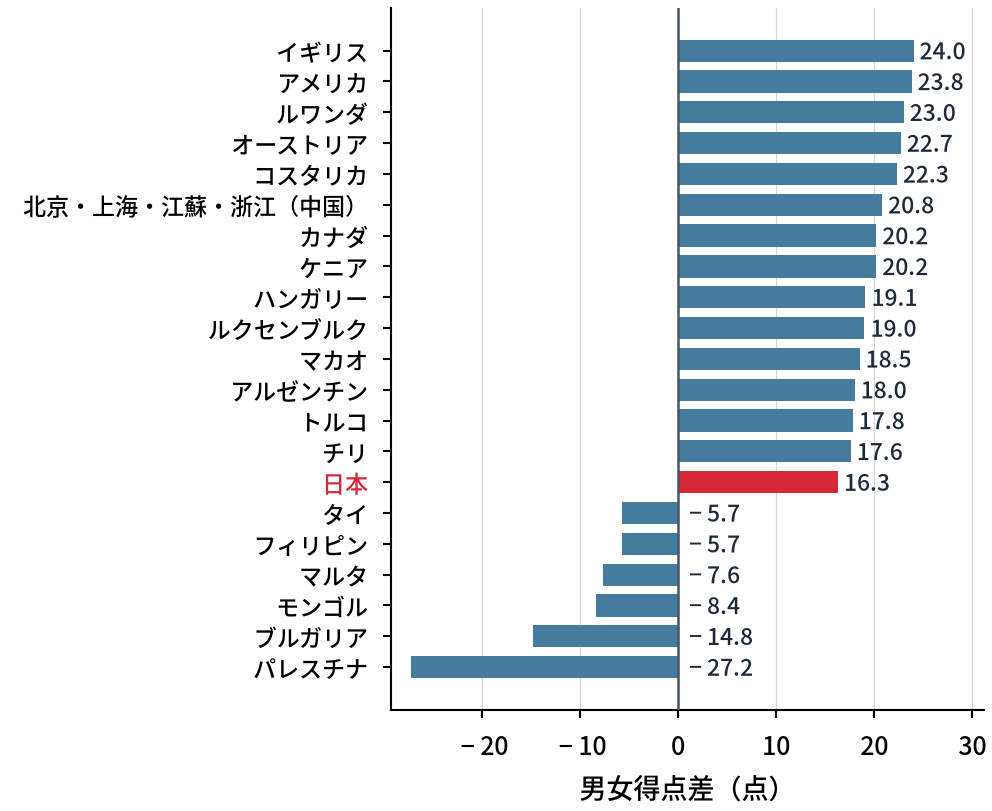
\includegraphics[width=\columnwidth]{chart_oecd_pisa2025_gender_gap.png}\caption{男女得点差の値の比較（上位・下位と日本を抜粋）．赤が日本}\end{figure}
\begin{figure}[t]\centering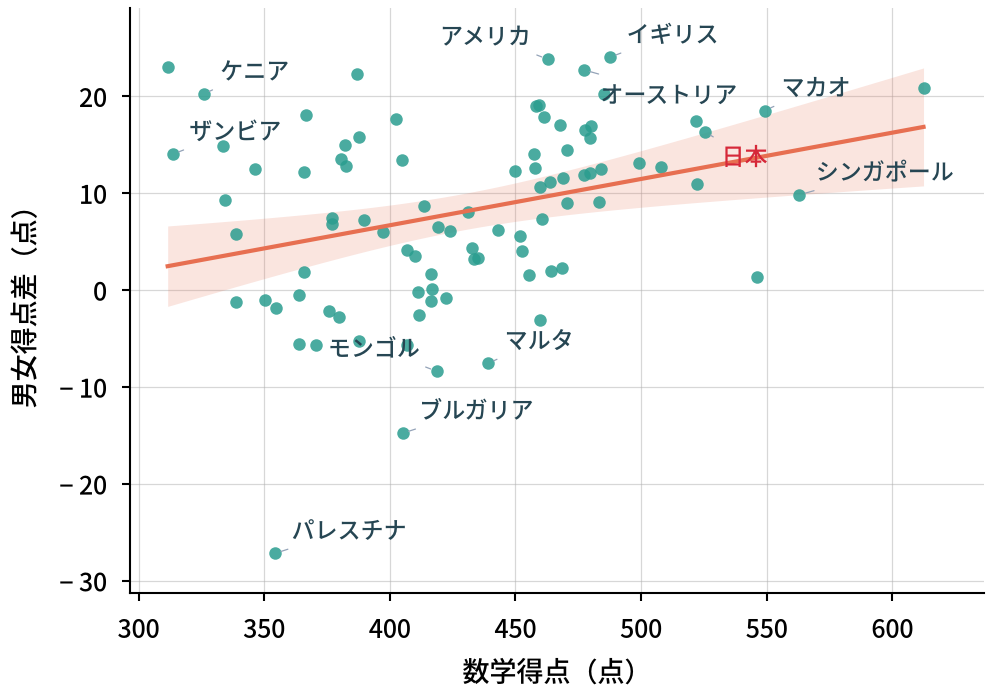
\includegraphics[width=\columnwidth]{chart_secondary_oecd_pisa2025_gender_gap.png}\caption{数学得点と男女得点差の関連（回帰直線と，その平均の95\%信頼区間の帯，n=90）}\end{figure}
\section{考察}
RQ1では，男女得点差が国・地域によって-27.2点から24.0点まで大きく異なり，多くは男子のほうが高かった．ただし女子のほうが高いと言える国・地域も7あり，一方向の現象ではない．日本は平均得点が高く，男子も女子も5番目で，差も大きい側にあるが，標準誤差が大きく，差が平均より大きいと断定できない．注意（*）のある6か国を除いても65対19で，日本は17番目，1か国ずつ除いても18か19番目であり，日本の位置は変わらなかった．平均得点の上位10を除いた80でも61対19で，差の偏りは残った（この分析には日本自身が含まれないので，日本の位置の確認には使えない）．RQ2の62は5\%水準を90回繰り返した結果で，補正すると，.05÷90とHolm法で44，偽発見率5\%のBenjamini-Hochberg法で60であり，基準によって44から62の幅がある．標準誤差の違いを考慮した異質性も大きく（Cochran Q=1046，自由度89，I²=91\%），差の幅は推定誤差だけでは説明できない．Hyde et al. (2008)が論じた「類似性」と整合するかは，得点の標準偏差に対する差の大きさを見る必要があり，本研究のデータでは判断できない．Else-Quest et al. (2010)が国による違いを扱ったことと，今回の国による差の幅は同じ問いに関わるが，同じ指標での比較ではない．

差の理由として，Guiso et al. (2008)の文化，Spencer et al. (1999)のステレオタイプ脅威，Blickenstaff (2005)の進路をめぐる議論が考えられる．いずれも仮説にとどまり，本研究のデータでは検証できない．集計値の関連は個々の生徒の因果を示さず（生態学的誤謬），Lindberg et al. (2010)が扱った時間的な傾向やOECD (2023)のPISA 2022との変化も見ていない．

限界は，(1)集計値のみで個人の因果を特定できないこと，(2)得点は標本調査の推定値で，学校に在籍する15歳に限られ，在籍率が男女で違う国では差が選抜の影響を受けうること（差の大きい側にルワンダなどが入っており，差は各国の15歳全体の差ではない），標準誤差が国ごとに異なり，国でない地域も同じ重みで数えていること，(3)注意（*）のある6か国を含むこと，(4)経済水準や学校の条件などの交絡を統制していないこと，(5)2025年の1時点であること，(6)90回の検定で多重比較の影響が残ること，である．教育現場で男女差に取り組む効果は，確かめられていない．
\section*{参考文献}
\begingroup\scriptsize\raggedright\interlinepenalty=10000 
\begin{list}{}{\setlength{\leftmargin}{1.5\zw}\setlength{\itemindent}{-1.5\zw}\setlength{\labelwidth}{0pt}\setlength{\labelsep}{0pt}\setlength{\itemsep}{1pt}\setlength{\parsep}{0pt}\setlength{\topsep}{0pt}\setlength{\listparindent}{0pt}}
\item BLICKENSTAFF, J. C. (2005) Women and science careers: Leaky pipeline or gender filter? Gender and Education, \textbf{17} (4) ：369-386.
\item ELSE-QUEST, N. M., HYDE, J. S. and LINN, M. C. (2010) Cross-national patterns of gender differences in mathematics: A meta-analysis. Psychological Bulletin, \textbf{136} (1) ：103-127.
\item GUISO, L., MONTE, F., SAPIENZA, P. and ZINGALES, L. (2008) Culture, gender, and math. Science, \textbf{320} (5880) ：1164-1165.
\item HYDE, J. S., LINDBERG, S. M., LINN, M. C., ELLIS, A. B. and WILLIAMS, C. C. (2008) Gender similarities characterize math performance. Science, \textbf{321} (5888) ：494-495.
\item LINDBERG, S. M., HYDE, J. S., PETERSEN, J. L. and LINN, M. C. (2010) New trends in gender and mathematics performance: A meta-analysis. Psychological Bulletin, \textbf{136} (6) ：1123-1135.
\item OECD (2023) PISA 2022 Results (Volume I): The State of Learning and Equity in Education. OECD Publishing, Paris. DOI: 10.1787/53f23881-en
\item OECD (2026) PISA 2025 Results (Volume I). OECD Publishing, Paris. DOI: 10.1787/73451bc5-en
\item SPENCER, S. J., STEELE, C. M. and QUINN, D. M. (1999) Stereotype threat and women's math performance. Journal of Experimental Social Psychology, \textbf{35} (1) ：4-28.
\end{list}\endgroup
\section*{Summary}
{\footnotesize\setlength{\parindent}{0pt}Using published PISA 2025 values, we organized the gender gap (male - female) in mathematical literacy across 90 countries and economies. The gap ranged from −27.2 to 24.0 points (unweighted mean 8.04), with 71 countries favoring males and 19 favoring females. In 62 (55 male, 7 female), the gap exceeded 1.96 times its standard error (approximately the 5\% level); 44 remained after a Bonferroni-type criterion (.05/90). Japan ranked 5th in mean score (525.4) and 19th from the top in the gap (16.3), but its standard error (5.7) was the second largest and its 95\% interval (5.1 to 27.5) included the mean gap, so its rank is uncertain. These are descriptions of country-level aggregates and do not imply causation for individual students.\par\smallskip KEYWORDS: PISA 2025, Mathematical Literacy, Gender Gap, International Comparison\par}
\medskip\noindent\fbox{\parbox{\dimexpr\columnwidth-2\fboxsep-2\fboxrule}{\footnotesize\gtfamily 【付記：生成AIによる自動執筆に関する開示】\\ 本論文は学生への教育目的で作成している．使用しているデータは公的オープンデータである．統計の算出はPythonで行い，文章は生成AI（Anthropic Claude等）を活用して作成した．記載した統計数値は元データに準拠しているが，教育学的な考察や提言の妥当性は，指導現場の実情に応じて，批判的に吟味してほしい．}}
\end{document}
